\chapter{Настройка NAT и DHCP-сервера}
\label{ch:nat-dhcp}

\section{Включение IP-форвардинга}
\label{sec:ipforward}

Открываем файл \texttt{/etc/sysctl.conf} и снимаем комментарий со строки,
отвечающей за перенаправление пакетов:

\begin{lstlisting}
nano /etc/sysctl.conf
# Снять комментарий со строки:
net.ipv4.ip_forward=1
\end{lstlisting}

% --- Скриншот: файл sysctl.conf с разкомментированной строкой ip_forward ---
\begin{figure}[h]
  \centering
  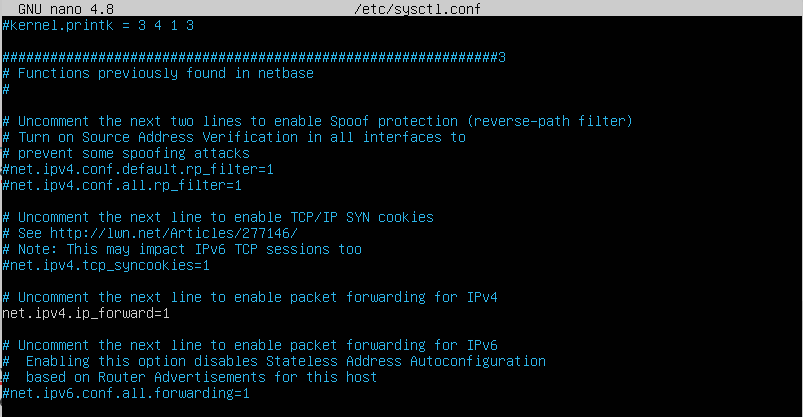
\includegraphics[width=0.85\textwidth]{img/08_sysctl_ipforward}
  \caption{Файл \texttt{/etc/sysctl.conf}: включён параметр \texttt{net.ipv4.ip\_forward=1}}
  \label{fig:sysctl}
\end{figure}

\section{Установка iptables-persistent}
\label{sec:iptables-persistent}

Для сохранения правил \texttt{iptables} между перезагрузками устанавливаем
пакет \texttt{iptables-persistent}. При установке система дважды запрашивает
подтверждение сохранения текущих правил~--- соглашаемся:

\begin{lstlisting}
apt-get update
apt install iptables-persistent
\end{lstlisting}

% --- Скриншот: диалог сохранения правил во время установки iptables-persistent ---
\begin{figure}[h]
  \centering
  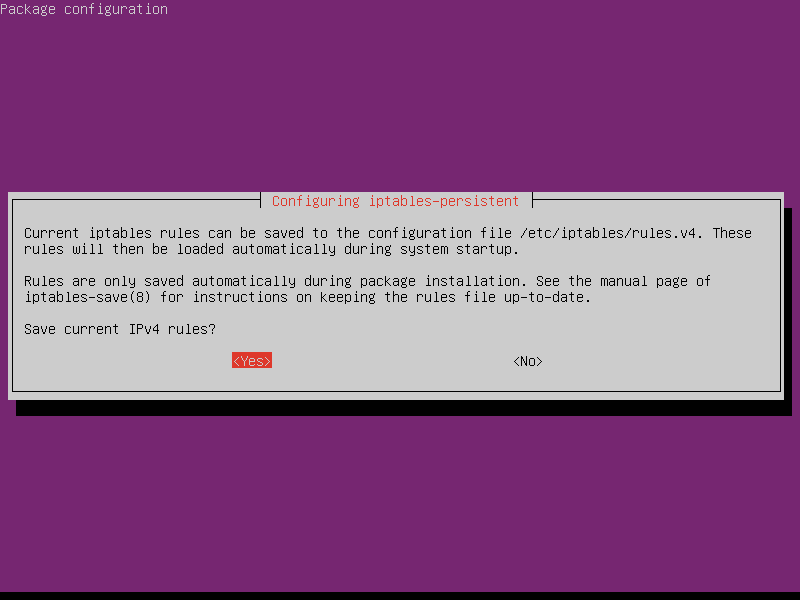
\includegraphics[width=0.85\textwidth]{img/09_iptables_persistent_dialog}
  \caption{Диалог сохранения правил при установке \texttt{iptables-persistent}}
  \label{fig:iptables-dialog}
\end{figure}

\section{Настройка правил iptables}
\label{sec:iptables-rules}

Создаём правила NAT и форвардинга:

\begin{lstlisting}
iptables -F
iptables -t nat -A POSTROUTING -o enp0s3 -j MASQUERADE
iptables -A FORWARD -i enp0s3 -o enp0s3 -j REJECT
iptables -I FORWARD -p tcp --tcp-flags SYN,RST SYN -j TCPMSS --clamp-mss-to-pmtu
\end{lstlisting}

Добавляем правила для перенаправления DNS-запросов внутренней сети
на сервер Google (\texttt{8.8.8.8}):

\begin{lstlisting}
iptables -t nat -A PREROUTING -i enp0s8 -p tcp --dport 53 -j DNAT \
    --to-destination 8.8.8.8:53
iptables -t nat -A PREROUTING -i enp0s8 -p udp --dport 53 -j DNAT \
    --to-destination 8.8.8.8:53
\end{lstlisting}

Сохраняем правила и перезагружаем сервер:

\begin{lstlisting}
iptables-save > /etc/iptables/rules.v4
reboot
\end{lstlisting}

% --- Скриншот: вывод iptables -L -n -v или iptables -t nat -L ---
\begin{figure}[h]
  \centering
  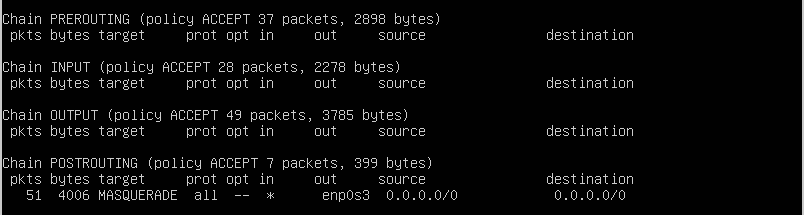
\includegraphics[width=0.85\textwidth]{img/10_iptables_rules}
  \caption{Созданные правила NAT (вывод \texttt{iptables -t nat -L})}
  \label{fig:iptables-rules}
\end{figure}

Правило \texttt{MASQUERADE} заменяет IP-адрес источника в исходящем пакете
на \texttt{10.0.2.15}. Правила \texttt{DNAT} перенаправляют DNS-запросы
внутренней сети на сервер Google.

\section{Установка и настройка DHCP-сервера}
\label{sec:dhcp-setup}

Устанавливаем пакет \texttt{isc-dhcp-server}:

\begin{lstlisting}
apt-get update
apt install isc-dhcp-server
\end{lstlisting}

\textbf{Указываем интерфейс}, на котором будет работать DHCP-сервер:

\begin{lstlisting}
nano /etc/default/isc-dhcp-server
# Редактируем строку:
INTERFACESv4="enp0s8"
\end{lstlisting}

% --- Скриншот: файл /etc/default/isc-dhcp-server с указанным INTERFACESv4 ---
\begin{figure}[h]
  \centering
  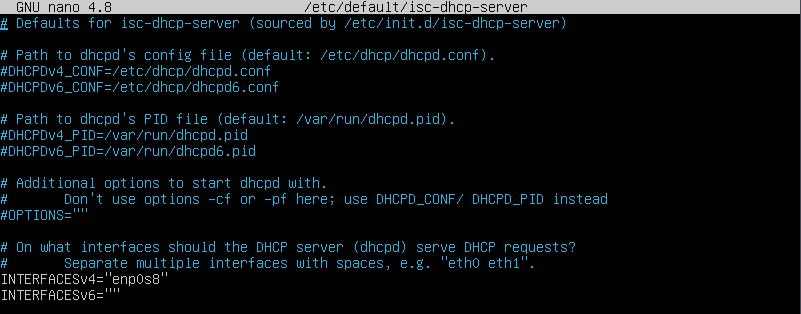
\includegraphics[width=0.85\textwidth]{img/11_dhcp_interfaces}
  \caption{Файл \texttt{/etc/default/isc-dhcp-server}: указан интерфейс \texttt{enp0s8}}
  \label{fig:dhcp-interfaces}
\end{figure}

\textbf{Подготовка конфигурационного файла} (предварительно делаем резервную
копию и очищаем оригинал):

\begin{lstlisting}
cp /etc/dhcp/dhcpd.conf /etc/dhcp/dhcpd.conf.example
echo "" > /etc/dhcp/dhcpd.conf
nano /etc/dhcp/dhcpd.conf
\end{lstlisting}

% --- Скриншот: содержимое файла dhcpd.conf в nano ---
\begin{figure}[h]
  \centering
  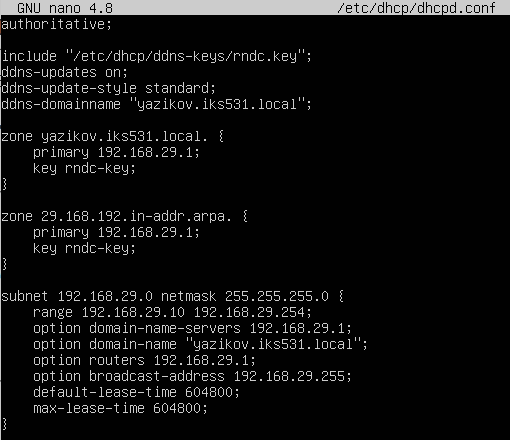
\includegraphics[width=0.85\textwidth]{img/12_dhcpd_conf}
  \caption{Конфигурационный файл \texttt{/etc/dhcp/dhcpd.conf}}
  \label{fig:dhcpd-conf}
\end{figure}

\textbf{Содержимое конфигурационного файла:}

\begin{lstlisting}
authoritative;
subnet 192.168.N.0 netmask 255.255.255.0 {
    range 192.168.N.10 192.168.N.254;
    option domain-name-servers 192.168.N.1;
    option routers 192.168.N.1;
    option broadcast-address 192.168.N.255;
    default-lease-time 604800;
    max-lease-time 604800;
}
\end{lstlisting}

Строка \texttt{authoritative;} означает, что данный сервер является
\textit{авторитетным} в сети. Время аренды задаётся в секундах
(\texttt{604800}~с~$= 7$~суток).

\textbf{Запуск и проверка сервиса:}

\begin{lstlisting}
service isc-dhcp-server start
service isc-dhcp-server status
\end{lstlisting}

% --- Скриншот: вывод service isc-dhcp-server status (статус active running) ---
\begin{figure}[h]
  \centering
  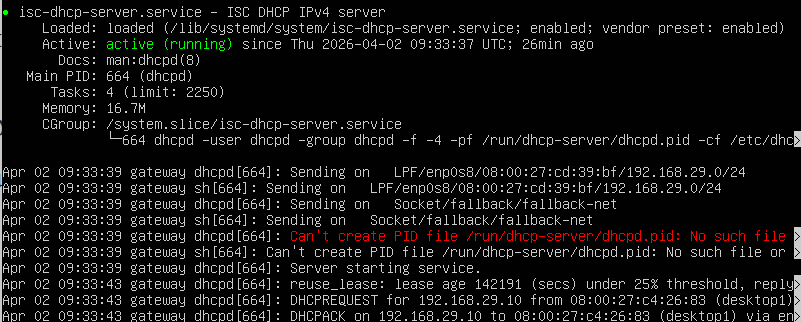
\includegraphics[width=0.85\textwidth]{img/13_dhcp_status}
  \caption{Статус сервиса \texttt{isc-dhcp-server}: \texttt{active (running)}}
  \label{fig:dhcp-status}
\end{figure}

В статусе должна присутствовать строка
\texttt{Active: active (running)}, а в логах~--- указание на прослушивание
интерфейса \texttt{enp0s8} с сетью \texttt{192.168.\cfgLabStudentN.0/24}.

\section{Резервирование IP-адреса по MAC}
\label{sec:dhcp-reservation}

При необходимости закрепить постоянный IP-адрес за конкретной машиной
в файл \texttt{/etc/dhcp/dhcpd.conf} добавляется следующая секция:

\begin{lstlisting}
host testhost {
    hardware ethernet 00:01:8a:e3:5e:92;
    fixed-address 192.168.N.51;
}
\end{lstlisting}

Где \texttt{hardware ethernet}~--- MAC-адрес сетевой карты клиента,
a \texttt{fixed-address}~--- IP-адрес, который будет выдаваться
исключительно данному устройству.

\section{Проверка выдачи адреса клиенту}
\label{sec:dhcp-verify}

На \texttt{Desktop1} переключаем получение адреса на <<автоматически>>.
Машина получает адрес из диапазона
\texttt{192.168.\cfgLabStudentN.10}--\texttt{192.168.\cfgLabStudentN.254}.
Просмотр выданных аренд:

\begin{lstlisting}
nano /var/lib/dhcp/dhcpd.leases
\end{lstlisting}

% --- Скриншот: Desktop1 получил IP от DHCP (настройки сети графического интерфейса или ip a) ---
\begin{figure}[h]
  \centering
  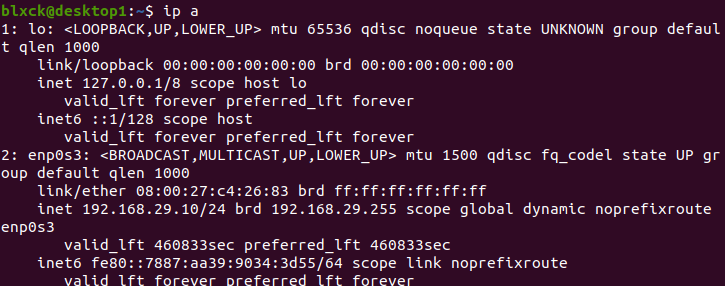
\includegraphics[width=0.75\textwidth]{img/14_desktop_dhcp_ip}
  \caption{Клиент Desktop1 получил IP-адрес от DHCP-сервера}
  \label{fig:dhcp-client}
\end{figure}

\textbf{Проверка связи и доступа в Интернет с клиента:}

\begin{lstlisting}
ping 192.168.N.1
ping ya.ru
\end{lstlisting}

% --- Скриншот: ping ya.ru с Desktop1 (Интернет работает) ---
\begin{figure}[h]
  \centering
  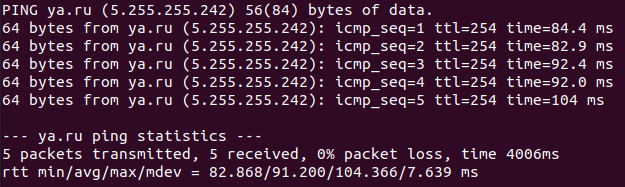
\includegraphics[width=0.85\textwidth]{img/15_ping_yaru_desktop}
  \caption{Проверка доступа в Интернет с \texttt{Desktop1} (\texttt{ping ya.ru})}
  \label{fig:ping-desktop}
\end{figure}

\section{Траблшутинг}
\label{sec:troubleshoot}

В случае возникновения проблем перезапускаем сервис и просматриваем
журнал системных событий:

\begin{lstlisting}
service isc-dhcp-server restart
service isc-dhcp-server status
tail -50 /var/log/syslog
\end{lstlisting}

% --- Скриншот: вывод tail -50 /var/log/syslog с примером ошибки (semicolon expected) ---
\begin{figure}[h]
  \centering
  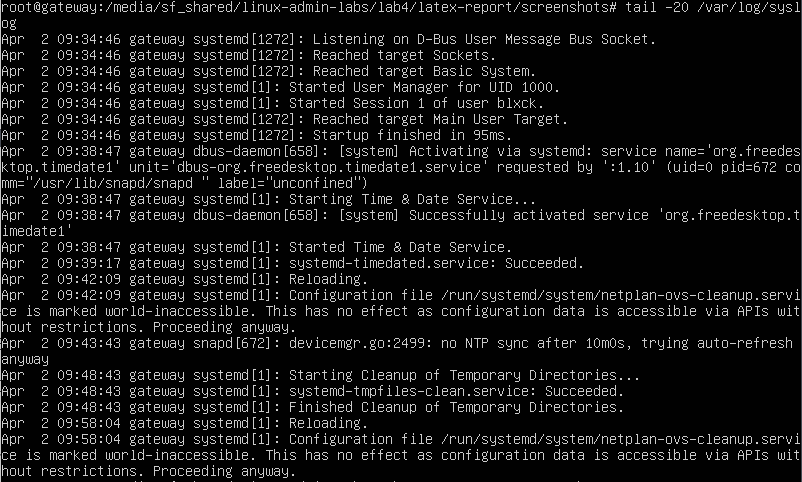
\includegraphics[width=0.85\textwidth]{img/16_syslog_error}
  \caption{Пример ошибки в \texttt{/var/log/syslog}: отсутствие точки с запятой в \texttt{dhcpd.conf}}
  \label{fig:syslog-error}
\end{figure}

Файл \texttt{/var/log/syslog} позволяет определить причину ошибки~---
например, пропущенную точку с запятой после \texttt{authoritative}
в конфигурационном файле DHCP-сервера.
